\documentclass[12pt, %
openright, 
oneside, %
%twoside, %TCC: Se seu texto tem mais de 100 páginas, descomente esta linha e comente a anterior
a4paper,    %
%english,   %
brazil]{facom-ufu-abntex2}

\usepackage[brazil]{babel}
\usepackage{graphicx}
\usepackage{minted}
\usepackage{hyperref}


% coisas relacionadas às cores do código:

\definecolor{dkgreen}{rgb}{0,0.6,0}
\definecolor{gray}{rgb}{0.5,0.5,0.5}
\definecolor{mauve}{rgb}{0.58,0,0.82}



\graphicspath{{figuras/}{pictures/}{images/}{./}} % where to search for the images

\newcommand{\blue}[1]{\textcolor{blue}{#1}}
\newcommand{\red}[1]{\textcolor{red}{#1}}


\autor{Pedro Henrique Bufulin de Almeida} %TCC
\data{2021}
\orientador{Pedro Frosi Rosa} %TCC
%\coorientador{Algum?} %TCC

% ---
% Informações de dados para CAPA e FOLHA DE ROSTO
% ---

\titulo{Sistema de vigilância \textit{\foreignlanguage{english}{open source}} e customizável} %TCC

\hypersetup{pdfkeywords={palavra 1}{palavra 2}{palavra 4}{palavra 4}{palavra 5}} %TCC

\begin{document}

\frenchspacing

% ----------------------------------------------------------
% ELEMENTOS PRÉ-TEXTUAIS
% ----------------------------------------------------------
%\pretextual
\imprimircapa
\imprimirfolhaderosto

% ---
% Inserir folha de aprovação
% ---
%
% \includepdf{folhadeaprovacao_final.pdf} %TCC: depois de aprovado o trabalho, descomente esta linha e comente o próximo bloco para incluir scan da folha de aprovação.
%
\begin{folhadeaprovacao}

	\begin{center}
		{\ABNTEXchapterfont\large\imprimirautor}

		\vspace*{\fill}\vspace*{\fill}
		{\ABNTEXchapterfont\bfseries\Large\imprimirtitulo}
		\vspace*{\fill}

		\hspace{.45\textwidth}
		\begin{minipage}{.5\textwidth}
			\imprimirpreambulo
		\end{minipage}%
		\vspace*{\fill}
	\end{center}

	Trabalho aprovado. \imprimirlocal, 01 de novembro de 2016: %TCC:

	\assinatura{\textbf{\imprimirorientador} \\ Orientador}
	\assinatura{\textbf{Professor}}% \\ Convidado 1} %TCC:
	\assinatura{\textbf{Professor}}% \\ Convidado 2} %TCC:
	%\assinatura{\textbf{Professor} \\ Convidado 3}
	%\assinatura{\textbf{Professor} \\ Convidado 4}

	\begin{center}
		\vspace*{0.5cm}
		{\large\imprimirlocal}
		\par
		{\large\imprimirdata}
		\vspace*{1cm}
	\end{center}

\end{folhadeaprovacao}
% ---

%%As seções dedicatória, agradecimento e epígrafe não são obrigatórias.
%%Só as mantenha se achar pertinente.

% ---
% Dedicatória
% ---
%\begin{dedicatoria}
%   \vspace*{\fill}
%   \centering
%   \noindent
%   \textit{Dedico a \lipsum[10]}  %TCC:
%   \vspace*{\fill}
%\end{dedicatoria}
% ---

% ---
% Agradecimentos
% ---
%\begin{agradecimentos}
%Agradeço a \lipsum[30]. %TCC:
%\end{agradecimentos}
% ---

% ---
% Epígrafe
% ---
%\begin{epigrafe}
%    \vspace*{\fill}
%	\begin{flushright}
%		\textit{``Alguma citação que ache conveniente? \lipsum[10]''} %TCC:
%	\end{flushright}
%\end{epigrafe}
% ---

\begin{resumo} %TCC:
	Os sistemas de vigilância carecem de soluções
	que sejam customizáveis. Apesar de existirem no mercado câmeras que fazem a gravação e o armazenamento de
	imagem, elas o fazem com com baixa resolução e limitações de espaço de memória severas. Mesmo os equipamentos
	de monitoramento mais sofisticados, como os que possuem reconhecimento de imagem, limitam o usuário de aprimorar
	essas funções por ter o \textit{\foreignlanguage{english}{software}} como \textit{\foreignlanguage{english}{closed source}}.
	Além disso, as soluções providas pela segurança pública ou privada, quando existem, podem usar as imagens
	coletadas para seus próprios benefícios, o que afeta a privacidade do indivíduo. Este trabalho propõe uma solução que seja
	fácil de implementar, com ferramentas prontas para uso e completamente customizável por ser \textit{\foreignlanguage{english}{open source}}.
	Dadas essas características, surge o chamado \textit{\foreignlanguage{english}{Self-Sovereign Camera System}} (SSCS)
	\vspace{\onelineskip}

	\noindent
	\textbf{Palavras-chave}: código  aberto, visão computacional, IP câmera, streaming multimídia.  %TCC:
\end{resumo}

\begin{resumo}[Abstract]

	Surveillance systems lack customizable solutions. Despite the existence of
	cameras on the market that handle both recording and storage of images, they do
	so at low resolution and with severe memory space limitations. Even the most
	sophisticated monitoring equipment, such as those with image recognition
	capabilities, restrict the user from enhancing these features due to the
	software being closed source. Furthermore, solutions provided by public or
	private security, when available, may use the collected images for their own
	benefit, affecting individual privacy. This work proposes a solution that is
	easy to implement, equipped with ready-to-use tools, and fully customizable as
	it is open source. Given these characteristics, the so-called Self-Sovereign
	Camera System (SSCS) emerges.

	\vspace{\onelineskip}
	\noindent
	\textbf{Keywords}: open source, computer vision, IP camera, multimedia streaming.
\end{resumo}

% ---
% inserir lista de ilustrações
% ---
\pdfbookmark[0]{\listfigurename}{lof}
\listoffigures*
\cleardoublepage
% ---

% ---
% inserir lista de tabelas
% ---
\pdfbookmark[0]{\listtablename}{lot}
\listoftables*
\cleardoublepage
% ---

% ---
% inserir lista de abreviaturas e siglas
% ---
\begin{siglas} %TCC: 

	\item[SSCS] Self-Sovereign Camera System
	\item[CAGR] Compound Annual Growth Rate
	\item[UML] Unified Modeling Language
	\item[AVC] Advanced Video Coding
	\item[HEVC] High Efficiency Video Coding
	\item[VMS] Video surveillance Management System
	\item[FPS] Frames Per Second
	\item[API] Application Programming Interface
	\item[ORM] Object-Relational Mapping
	\item[DVR] Digital Video Recorder
	\item[NVR] Network Video Recorder
	\item[REST] Representational State Transfer
	\item[HSL] HTTP Live Streaming
	\item[RTSP] Real-time Streaming Protocol
	\item[SDP] Session Description Protocol
	\item[RTP] Real-time Transport Protocol
	\item[AU] Access Unit
	\item[NALU] Network Abstraction Layer Unit
	\item[WebRTC] Web Real-time Communication
	\item[SRT] Secure Reliable Transport
	\item[RTMP] Real Time Messaging Protocol
	\item[LBPH] Local Binary Patterns Histogram

\end{siglas}
% ---

%% ---
%% inserir lista de símbolos, se for adequado ao trabalho. %TCC:
%% ---
%\begin{simbolos}
%  \item[$ \Gamma $] Letra grega Gama
%  \item[$ \Lambda $] Lambda
%  \item[$ \zeta $] Letra grega minúscula zeta
%  \item[$ \in $] Pertence
%\end{simbolos}
%% ---

% ---
% inserir o sumario
% ---
\pdfbookmark[0]{\contentsname}{toc}
\tableofcontents*
\cleardoublepage
% ---

% ----------------------------------------------------------
% ELEMENTOS TEXTUAIS
% ----------------------------------------------------------
\textual

% ----------------------------------------------------------
% Introdução
% ----------------------------------------------------------

\chapter[Introdução]{Introdução}
%TCC:
% Contextualização, problema, hipótese, objetivo geral, objetivos específicos, justificativa e resultados esperados.
Em 2019 foi estimado que existem 200 milhões de câmeras de vigilância na China
e na última década, avanços tecnológicos tornaram essas câmeras ainda mais
eficientes em monitorar 1.4 bilhões de chineses. Ainda segundo o autor, o
reconhecimento de rostos por câmeras começou a ser uma realidade em 2010 quando
pesquisadores descobriram algoritmos de deep learning usados para reconhecer
imagens e voz. Esses algoritmos podem também inferir em tempo real a quantidade
e a densidade de pessoas numa dada imagem \cite{qiang2019road}.

Esta intensificação do uso da tecnologia de vigilância não se limita à China;
ou está se tornando ou já é a realidade em muitos outros países. De acordo com
um relatório da Market Research Future \cite{Gupta2018}, a América do Norte é
atualmente líder em termos de participação de mercado de câmeras de CCTV,
detendo 28,5\% do mercado global, seguida pela Europa com 18,3\%. Este domínio
é reflexo de um mercado de vigilância por vídeo que tem mostrado crescimento
substancial: avaliado em 45,9 bilhões de dólares em 2021, este mercado tem uma
projeção de crescimento para 110,2 bilhões de dólares até 2030, com uma taxa
composta anual de crescimento (CAGR) de 11,6\% para o período de 2022 a 2030.
Esses dados evidenciam não apenas a escala atual da indústria de vigilância,
mas também sua trajetória ascendente, realçando a importância de abordar
questões de privacidade e segurança em um contexto tão amplo e em rápido
crescimento.

À medida que o mercado de vigilância por vídeo se expande,
os sistemas associados também se tornam progressivamente mais complexos e de maior alcance.
Isso demonstra a necessidade de infraestruturas mais robustas e eficientes.
Nesse contexto, é intrigante observar que as complicações técnicas enfrentadas pelos
sistemas de vigilância têm muitas semelhanças com aquelas encontradas em plataformas de
streaming de vídeo. Ambos os tipos de
sistemas têm uma dependência substancial de infraestruturas distribuídas para
assegurar a prestação de serviços em tempo real, de maneira eficaz e confiável.

Entretanto, a privacidade dos indivíduos não é uma preocupação primária dos
principais provedores desse tipo de serviço. Nesse contexto, tecnologias de
código aberto podem oferecer uma solução, pois permitem que qualquer pessoa
verifique se o software tratando a segurança e a privacidade de maneira
adequada \cite{mardjan2016open}.

Considerando-se a necessidade de criar uma solução que traga os benefícios da
vigilância com as funcionalidades modernas de reconhecimento de imagem,
armazenamento e mantendo a privacidade individual, surge neste trabalho a
proposta da construção de um software de vigilância.

\section{Objetivos}

O propósito deste trabalho é projetar um sistema de monitoramento integralmente
sustentado por software livre, com capacidade de integração com uma ampla
variedade de dispositivos de hardware. Este sistema oferecerá visualização em
tempo real de imagens de câmeras, incorporando algoritmos de visão
computacional para análise destas. Será possível armazenar e buscar vídeos,
utilizando critérios identificados pelos algoritmos. Uma das grandes virtudes
do projeto é sua adaptabilidade: ele é projetado para permitir a inclusão de
novas funcionalidades, como notificações de eventos, e a modificação de
características existentes. Por exemplo, o armazenamento pode ser configurado
para ser local ou em nuvem, e o processamento para reconhecimento de imagens
pode ocorrer tanto em transmissões ao vivo quanto em vídeos arquivados. Para
facilitar a implementação e personalização do sistema, será disponibilizada uma
documentação abrangente, delineando várias opções de uso para satisfazer as
distintas necessidades dos usuários.

\subsection{Objetivos específicos}

Os objetivos específicos envolvem:

\begin{itemize}
	\item Desenvolver todo o software com código aberto e mantê-lo publicamente
	      disponível no Github.
	\item Usar a conteinerização como estratégia para conseguir portabilidade entre
	      vários hardwares e sistemas operacionais diferentes.
	\item Implementar uma funcionalidade de visualização em tempo real de imagens
	      provenientes de câmeras.
	\item Incorporar algoritmos de visão computacional para análise e processamento das
	      imagens em tempo real.
	\item Projetar e desenvolver um módulo de armazenamento flexível, permitindo opções
	      tanto locais quanto em nuvem.
	\item Habilitar a busca de vídeos com critérios baseados nas identificações
	      realizadas pelos algoritmos de visão.
	\item Possibilitar a customização do sistema, incluindo a adição de novas
	      funcionalidades como notificações de eventos.
	\item Adaptar o sistema para permitir variações nos métodos de reconhecimento de
	      imagens, seja em transmissões ao vivo ou em vídeos arquivados.
	\item Escrever testes automatizados e \textit{\foreignlanguage{english}{benchmarks}}
	      para manter a qualidade do software e das soluções em um nível aceitável.
	\item Produzir uma documentação detalhada e abrangente, facilitando a implementação,
	      personalização e manutenção do sistema por parte dos usuários.
\end{itemize}

\section{Justificativa}

Ainda que existam várias soluções disponíveis em hardware, elas não se integram
facilmente umas com as outras. Por vezes usam protocolos e formatos de arquivo
diferentes, excluindo alguns softwares de se integrarem com o hardware. Outras
vezes é o contrário: o software não se adapta ao hardware, e mesmo se existe um
que seja possível integrar, ele não tem as funcionalidades desejadas. Portanto,
faz sentido um software customizável que possa se adaptar as necessidades do
usuário e que crie uma fundação para criar novas funções de vigilância.

\section{Resultados esperados}

 (não sei se é necessária essa parte, já que temos todos os objetivos específicos postulados logo acima)

\chapter{Fundamentação Teórica}

Neste capítulo, são apresentadas as tecnologias e os conceitos que serão
empregados ao longo da execução deste projeto. Esses conceitos estão
relacionados à arquitetura do sistema que será desenvolvido, aos protocolos,
técnicas de reconhecimento de imagem, compressão, técnicas de software e demais
elementos necessários para a materialização da solução proposta.

\section{Elementos genéricos de um sistema de multimídia}

A figura abaixo mostra um sistema de cliente-servidor para transmissão de dados
de multimídia. Na origem, tem-se a gravação comprimida, codificada e armazenada
no dispositivo de armazenamento, como um disco rígido, por exemplo. Em seguida,
por meio de algum software de mídia, esses arquivos são requisitados por
usuários e entregues de acordo. Uma Network Interface Card (NIC na figura)
então usa um protocolo de transmissão via rede para entregar os dados de
multimídia para o cliente (tais como RTMP, HLS, RTSP, WebRTC), onde eles são
primeiramente armazenados na memória principal ou disco e eventualmente
decodificados e apresentados ao usuário.

\begin{figure}[!ht]
	\centering
	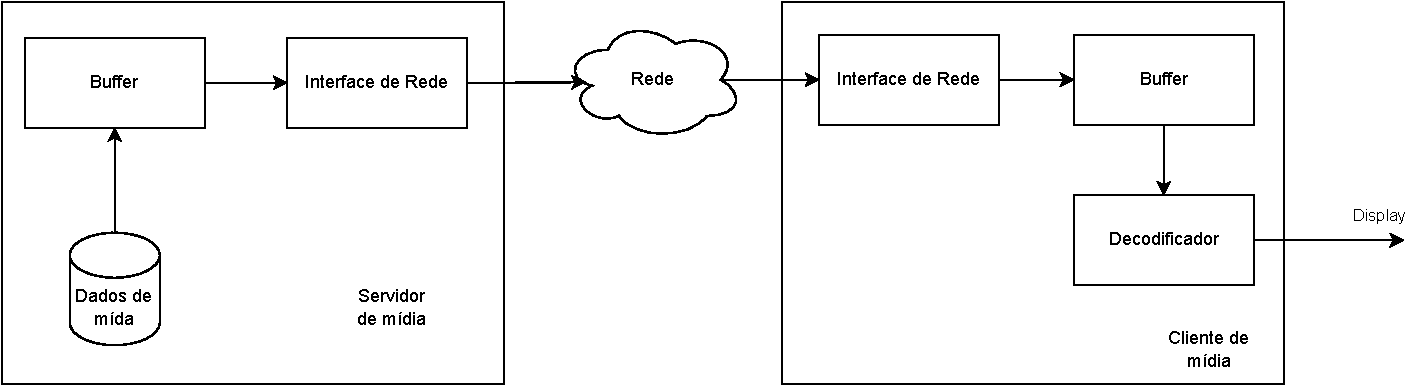
\includegraphics[width=1\linewidth]{media_fundamentals.pdf}
	\caption[Representação de um arquitetura de tempo real genérica]{Arquitetura genérica de transmissão em tempo real}
	\label{fig:graficosVariandoTamanhoRede}
\end{figure}

Uma característica única deste modelo de sistema é que os componentes do
sistema envolvidos trabalham em conjunto no processo de entrega de dados.
Assim, um problema em qualquer um dos componentes do sistema pode degradar o
desempenho de toda a cadeia.

\subsection{Dados de mídia}

O 'multi' em multimídia refere-se a múltiplos meios de comunicação do mesmo
tipo ou de tipos diferentes que são criados, entregues e apresentados juntos.
Existem muitos tipos diferentes de mídia, desde o texto simples mais básico,
até texto formatado, gráficos, imagens, áudio, vídeo ou até mesmo informações
táteis. Podemos classificar amplamente esses diversos tipos de mídia em duas
categorias principais, especialmente no contexto da entrega de dados
multimídia: mídias discreta ou contínuas.

As discretas referem-se às que não possuem nenhum requerimento explícito de
tempo de apresentação. Por exemplo, buscar na rede para exibi-la no navegador.
Dependendo da largura de banda disponível, o navegador pode levar um tempo
largamente variável até receber a imagem antes que ela seja decodificada e em
seguida apresentada. Obviamente, é preferível que esse processo seja o mais
breve o possível, mas desde que os dados da imagem sejam recebidos
corretamente, renderizados e apresentados, a requisição é considerada bem
sucedida. Em outras palavras, não há restrição inerente nos dados de mídia que
exigem a apresentação em um prazo de tempo ou limite de atraso. É por isso que
o tráfego de rede criado pela entrega de mídia discreta é chamado tráfego
elástico. Esse nome refere-se à possibilidade de tolerar variações em tempo de
atraso.

As contínuas, em contrapartida, possuem um prazo de tempo para a apresentação
embarcados nos seus dados de mídia. Por exemplo, dados de vídeo estão
geralmente codificados em quadros que precisam ser apresentados sequencialmente
em uma frequência específica como 25 FPS. Portanto, para apresentar o vídeo
corretamente é necessário não só receber os dados corretamente como também
sequenciar de acordo com os tempos especificados. Falhas no sequenciamento
podem causar degradações perceptíveis na qualidade do vídeo (movimentação lenta
ou fatiada) mesmo se a transmissão foi bem sucedida. Nesse sentido, tráfego de
rede proveniente de mídia contínua também é conhecido como tráfego
não-elástico, pois precisa manter o tempo íntegro. \cite{lee2005scalable}

% \section{Sistema distribuído aberto}

% Esta arquitetura é a que levarei em consideração na implementação do projeto. O
% servidor que será implementado utilizando um microcomputador contem a câmera e
% sistema operacional para realizar o processamento e transmissão dos dados de
% multimídia. Outra alternativa seria o microcomputador apenas enviar os fluxo de
% vídeo para um terceiro servidor que faria o processamento da imagem caso a
% capacidade daquele não seja suficiente, resultando em um sistema distribuído.
% Essa outra abordagem também respeita a arquitetura citada acima.

% \section{Framework de desenvolvimento front end}

% Como é de se esperar, um sistema que permite a visualização em tempo real
% necessitará de um meio para apresentar ao usuário as saídas e o resultado do
% processamento delas. Como se trata de um sistema de segurança, o mais viavel é
% que o usuário sempre tenha em mãos o dispositivo que fornece a imagem, ou seja,
% o \emph{smartphone}. Portanto, faz sentido utilizar um \emph{framework} que
% permita a criação de um front end mobile. Além disso, a aplicação resultante
% deverá ser replicável em múltiplos dispositivos, para que o usuário não seja
% tolhido por não ter o meio adequado. Dadas essas condições, o \emph{framework}
% que satisfaz elas é o \emph{React Native}

% O React Native é um framework de desenvolvimento mobile híbrido (iOS e Android
% simultâneamente) voltado para a construção de interfaces de usuário criado pelo
% facebook, utilizando \emph{javascript} com a linguagem de programação e
% compilando-o de forma que seja executável pela plataforma nativa. Vale lembrar
% que o React Native não é uma solução \emph{full-stack} que vai lidar com tudo
% desde o banco de dados à atualizações em tempo real de \emph{web sockets}. Ele
% é simplesmente a \emph{View layer} da aplicação. \cite{boduch2017react}

\section{Técnicas de reconhecimento de imagem}

\subsection{Subtração de Fundo baseada em Modelos de Mistura Gaussiana}

A subtração de fundo desempenha um papel crucial no pré-processamento de muitas
aplicações de visão computacional. Por exemplo, em um contador de visitantes,
onde uma câmera estática registra a entrada e saída de pessoas em uma sala, ou
em uma câmera de tráfego que extrai informações dos veículos, há a necessidade
de isolar com precisão as pessoas ou veículos em movimento do fundo estático.
Nesses cenários, é necessário encontrar as imagens dinâmicas, separando-as das
estáticas.

Se no cenário houver uma imagem apenas do fundo, ou seja, de uma sala sem
visitantes ou uma estrada sem veículos, o reconhecimento é tecnicamente mais
fácil. Basta subtrair a nova imagem do fundo. Porém, na maioria dos casos, a
imagem não é regular, então é preciso extrair o fundo das imagens existentes.
Essa tarefa fica mais complicada quando há sombras nos objetos em movimento,
pois a sombra se move junto com o objeto e algoritmos que não levam isso em
consideração marcam a sombra como plano primário. \cite{opencv_bgsubtraction}

Nesse sentido, como a maioria dos algoritmos de subtração de fundo têm sua
performance afetada pela disposição da iluminação do cenário, pesquisadores
desenvolveram um método baseado na mistura de Gaussianos para lidar com esse
problema. Nesse método, no lugar de modelar os valores de todos os pixels em um
tipo particular de distribuição, os valores de um pixel em particular são
modelados como uma mistura de Gaussianos. Baseado na persistência e variância
de cada um dos Gaussianos da mistura, é possível determinar quais Gaussianos
correspondem à cores do fundo. Valores de pixel que não se encaixam nas
distribuições do fundo são considerados como primeiro plano, até que um
Gaussiano inclua-as con evidências consistentes e suficientes.

Assim, essa técnica se adapta para lidar com robustez à mudanças na iluminação,
movimentos repetitivos de elementos em cena, rastreamento através de regiões
desordenadas, objetos de movimento lento e introdução ou remoção de objetos da
cena. Objetos que se movem lentamente levam mais tempo para serem incorporados
ao fundo, porque a cor deles tem uma variação maior do que a do fundo. Além
disso, variações repetitivas são aprendidas, e um modelo para a distribuição de
fundo é geralmente mantido, mesmo que temporariamente substituído por outra
distribuição, o que leva a uma recuperação mais rápida quando os objetos são
removidos. \cite{784637}

\begin{figure}[!ht]
	\centering
	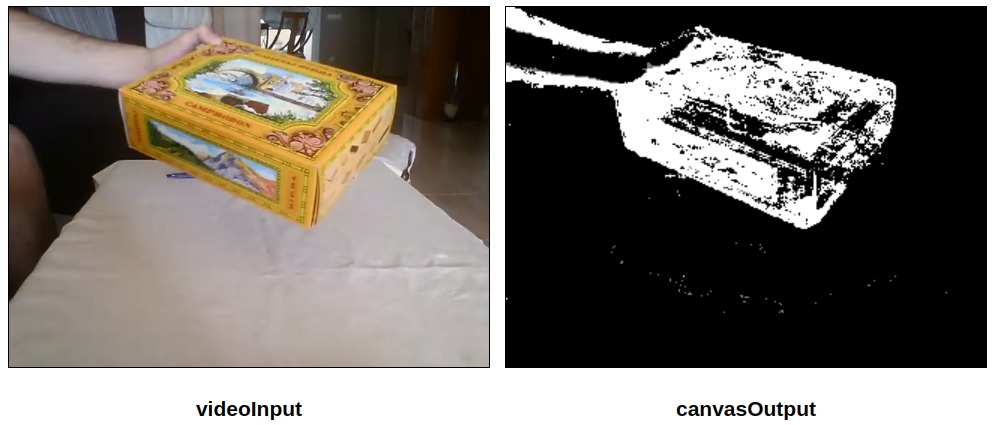
\includegraphics[width=0.7\linewidth]{background_subtraction.jpeg}
	\caption[Aplicação da técnica de subtração de fundo baseada em modelos de Mistura Gaussiana]{Aplicação da técnica de subtração de fundo baseada em modelos de Mistura Gaussiana}
	\label{fig:graficosVariandoTamanhoRede}
\end{figure}

\subsection{Detecção de objetos usando classificadores em cacata baseados em características de haar}

Neste método, utiliza-se aprendizado de máquina, onde uma função de cascata é
treinada a partir de um grande número de imagens positivas (contendo o objeto
de interesse) e negativas (sem o objeto de interesse). Nisso, as
características Haar, inspiradas nas wavelets de Haar, são usadas para
encontrar padrões visuais que diferenciam o objeto de interesse do restante da
imagem.

Essas características haar são simples retângulos de 3 tipos. A de dois
retângulos, onde o valor dessa é atribuído calculando-se a diferença entre a
soma dos pixels dentro de duas regiões retangulares de mesmo tamanho e forma,
adjacentes horizontalmente ou verticalmente. A de três retângulos calcula a
soma dentro de dois retângulos externos subtraindo a soma em um retângulo
central. Por último, uma característica de quatro retângulos calcula a
diferença entre pares de retângulos diagonais.

\begin{figure}[!ht]
	\centering
	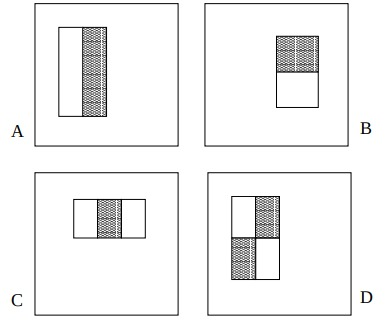
\includegraphics[width=0.7\linewidth]{haar_features.jpeg}
	\caption[Exemplos de características Haar mostradas em uma janela de detecção]{Exemplos de características Haar mostradas em uma janela de detecção}
	\label{fig:graficosVariandoTamanhoRede}
\end{figure}

As características Haar também podem ser calculadas rapidamente graças ao uso
de uma representação intermediária para a imagem chamada de imagem integral,
que permite a soma de valores de intensidade em áreas retangulares da imagem de
forma eficiente. Estas características são simples, mas extremamente eficazes
na captura de bordas, linhas e mudanças de textura em imagens.

A arquitetura em cascata do classificador também acrescenta na velocidade do
método. Cada estágio da cascata utiliza um conjunto de características Haar
para determinar se uma determinada região da imagem deve continuar sendo
processada pelas etapas subsequentes. As regiões que são prontamente
identificadas como não contendo o objeto são descartadas, reduzindo
significativamente o volume de cálculos necessários para a detecção.

Este método mostrou-se particularmente eficaz na detecção de rostos em tempo
real, mas também pode ser adaptado para a detecção de outros tipos de objetos.
A capacidade de operar em tempo real e com precisão tornou essa técnica um
marco na área de visão computacional, abrindo caminho para aplicações práticas
em segurança, interação humano-computador e outras áreas. \cite{990517}

\section{Arquitetura de microsserviços}

Explicar aqui o que são microsseviços e como eles funcionam. Fazer talvez uma
comparação em relação à uma monolito

\section{Arquitetura Monolítica}

Explicar aqui como funciona uma arquitetura monolítica e quais as desvantagens
e vantagens em relação ao microsserviço.

\section{Banco de dados relacional}

\section{Protoclo RTSP}

O Real-time Streaming Protocol (RTSP) é um protocolo da camada de aplicação
projetado para controlar a entrega de dados de mídia (por exemplo, reproduzir,
pausar e buscar) com informações de tempo embutidas, como áudio e vídeo. O
protocolo é independente do protocolo de camada inferior. Assim, o RTSP pode
ser transmitido por meio de TCP, UDP ou outros protocolos de transporte. A
sintaxe do RTSP compartilha muitas semelhanças com o HTTP/1.1, simplificando
assim a implementação e a implantação. No entanto, além das semelhanças de
sintaxe, o RTSP difere do HTTP em muitos aspectos importantes.

Primeiro, ao contrário do HTTP, o RTSP é um protocolo com estado, exigindo que
o host mantenha informações de estado de uma sessão de streaming em várias
requisições RTSP. Segundo, tanto o servidor quanto o cliente RTSP podem emitir
requisições RTSP. Finalmente, os dados de mídia devem ser entregues fora do
canal principal, ou seja, usando um protocolo separado, como, mas não limitado
a, o Protocolo de Transporte em Tempo Real (RTP).

Em uma aplicação de streaming típica (veja a figura abaixo), o cliente primeiro
obterá um arquivo de descrição de apresentação usando métodos fora do canal
principal (por exemplo, através da web usando HTTP). O arquivo de descrição de
apresentação descreve uma ou mais apresentações, cada uma composta por uma ou
mais transmissões de mídia sincronizadas. O arquivo de descrição de
apresentação também contém propriedades das transmissões de mídia, como o
formato de codificação, para permitir que o cliente selecione e se prepare para
a reprodução da mídia. Cada transmissão de mídia controlável é identificada por
uma URL RTSP separada, que é semelhante à URL HTTP no sentido de que identifica
o servidor que hospeda a transmissão de mídia e o caminho lógico que identifica
a transmissão de mídia. Observe que as transmissões de mídia em uma
apresentação podem vir de vários servidores e cada transmissão é controlada por
meio de uma sessão RTSP separada. \cite{rfc2326}

\begin{figure}[!ht]
	\centering
	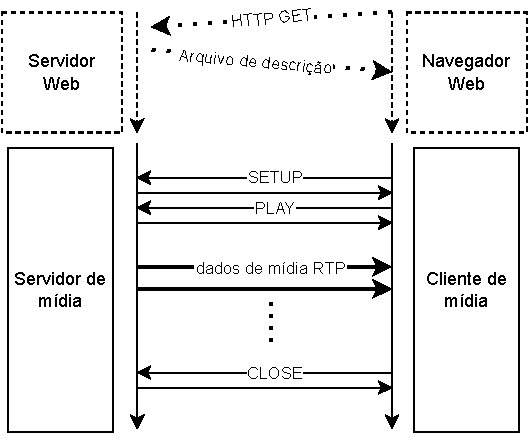
\includegraphics[width=0.8\linewidth]{rtsp.pdf}
	\caption[Diagrama RTSP]{Transmissão de mídia usando o RTSP, início ao fim. }
	\label{fig:rtspDiagram}
\end{figure}

\section{Diagrama UML de Componentes}

O diagrama de componentes é uma ferramenta da UML (Unified Modeling Language).
Ele tem como objetivo visualizar a organização e as relações entre diferentes
componentes em um sistema de software. Enquanto outros diagramas focam na
funcionalidade do sistema, o diagrama de componentes se concentra no aspecto
estrutural.

Um diagrama de componentes representa partes modulares de um sistema, chamadas
de componentes. Estes componentes podem ser físicos (como bibliotecas, módulos,
arquivos) ou conceituais e estão conectados através de interfaces. Estas
interfaces são os pontos de interação entre os componentes.

Características dos diagramas de componentes:
\begin{itemize}
	\item Mostram as dependências entre os componentes.
	\item Identificam as interfaces que conectam os componentes.
	\item Auxiliam na modularização e reutilização de software.
	\item Oferecem uma visão da arquitetura do sistema.
\end{itemize}

Ao trabalhar com diagramas de componentes, as equipes podem compreender melhor
a estrutura do sistema e identificar áreas para atenção ou desenvolvimento.

Abaixo, um exemplo de um componente e suas partes:

\begin{figure}[!ht]
	\centering
	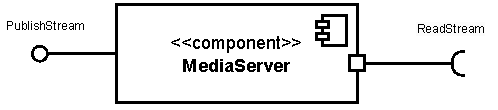
\includegraphics[width=0.8\linewidth]{example_diagram.pdf}
	\caption[Componente de exemplo]{Componente, provendo uma interface e com requerimento de outra}
	\label{fig:graficosVariandoTamanhoRede}
\end{figure}

O componente é representado pela estrutura retangular. O ícone no topo direito
do retângulo é opcional, sendo uma especificação do UML 1.4. Na Figura, o
círculo à esquerda com a legenda PublishStream indica uma interface provida, e
o semicírculo indica uma interface requerida.

Uma interface fornecida é aquela que é realizada diretamente pelo próprio
componente, ou realizada por um dos classificadores que implementam o
componente, ou ainda fornecida por uma porta pública do componente. Na notação
de pirulito, temos a interface fornecida do componente. No exemplo, o
componente de MediaServer fornece (implementa) a interface de PublishStream.

Uma interface necessária é aquela designada por uma dependência de uso do
próprio componente, ou designada por uma dependência de uso de um dos
classificadores que implementam o componente, ou ainda é exigida por uma porta
pública do componente. No exemplo, o componente MediaServer requer a interface
ReadStream.

O pequeno quadrado na linha é uma porta, e ela indica que a interface faz parte
não do componente em si mas de um de seus componentes internos encapsulados.

\section{Versionamento Semântico (SEMVER)}

O \textit{SEMVER}, abreviação de Versionamento Semântico, é uma convenção de
nomenclatura usada para gerenciar e comunicar eficazmente as mudanças em
versões de software. Ele cria uma maneira compreensível de representar as
mudanças em software através do número de sua versão.

A estrutura básica de um número de versão SEMVER é \textit{MAJOR.MINOR.PATCH},
onde:

\begin{itemize}
	\item \textit{MAJOR} é incrementado para mudanças incompatíveis que requerem que o usuário faça algo diferente.
	\item \textit{MINOR} é incrementado quando são feitas adições em um modo compatível, ou seja, quando funcionalidades são adicionadas sem alterar o comportamento das funcionalidades existentes.
	\item \textit{PATCH} é incrementado após correções de bugs que são compatíveis e não afetam o funcionamento global do software de maneira significativa.
\end{itemize}

Além destes três números principais, o SEMVER também permite a adição de
etiquetas pré-lançamento e de build, que podem ser usadas para representar
versões alfa, beta, candidatas a lançamento, entre outros.

O principal benefício de adotar o \textit{SEMVER} é a clareza. Ao olhar para o
número de versão de um software, os desenvolvedores podem rapidamente entender
a natureza e a magnitude das mudanças, facilitando decisões sobre a atualização
ou integração de dependências. \cite{semver}

\section{Daemon}

Um daemon é um processo em segundo plano que normalmente é executado
indefinidamente. O sistema operacional UNIX depende de muitos processos daemon
para realizar tarefas rotineiras (e não tão rotineiras). No ambiente
operacional Solaris, por exemplo, o daemon \texttt{pageout} gerencia a
paginação para o gerenciamento de memória. O \texttt{in.rlogind} lida com
solicitações de login remoto. Outros daemons lidam com correio, transferência
de arquivos, estatísticas e solicitações de impressora, para citar alguns.
\cite{kay2004unix}

\section{Princípios SOLID}

Os princípios SOLID, nos dizem como organizar nossas funções e estruturas de
dados em classes e como essas classes devem estar interconectadas. O uso da
palavra "classe" não implica que esses princípios se aplicam apenas ao software
orientado a objetos. Uma classe é simplesmente um agrupamento acoplado de
funções e dados. Todo sistema de software tem esses agrupamentos, quer sejam
chamados de classes ou não. Os princípios SOLID se aplicam a esses
agrupamentos. O objetivo dos princípios é a criação de estruturas de software
de nível médio que são fáceis de entender, formam a base de componentes que
podem ser usados em muitos sistemas software.

A história dos princípios SOLID é longa. Comecei a montá-los no final dos anos
1980, enquanto debatia princípios de design de software com outras pessoas no
USENET (um tipo primitivo de Facebook). Ao longo dos anos, os princípios
mudaram e evoluíram. Alguns foram excluídos. Outros foram mesclados. Ainda
outros foram adicionados. O agrupamento final estabilizou-se no início dos anos
2000, embora eu os tenha apresentado em uma ordem diferente.

\begin{itemize}
	\item \textbf{SRP: Princípio da Responsabilidade Única}\\
	      Um corolário ativo da lei de Conway: A melhor estrutura para um sistema de software é fortemente influenciada pela estrutura social da organização que o utiliza, de forma que cada módulo de software tenha uma, e apenas uma, razão para mudar.

	\item \textbf{OCP: Princípio Aberto-Fechado}\\
	      Bertrand Meyer tornou este princípio famoso na década de 1980. Em essência, para que os sistemas de software sejam fáceis de alterar, eles devem ser projetados para permitir que o comportamento desses sistemas seja alterado pela adição de novo código, em vez de alterar o código existente.

	\item \textbf{LSP: Princípio da Substituição de Liskov}\\
	      A famosa definição de subtipos de Barbara Liskov, de 1988. Em resumo, este princípio diz que para construir sistemas de software a partir de peças intercambiáveis, essas peças devem aderir a um contrato que permita que sejam substituídas umas pelas outras.

	\item \textbf{ISP: Princípio da Segregação da Interface}\\
	      Este princípio aconselha os designers de software a evitar depender de coisas que eles não usam.

	\item \textbf{DIP: Princípio da Inversão de Dependência}\\
	      O código que implementa políticas de alto nível não deve depender do código que implementa detalhes de baixo nível. Pelo contrário, os detalhes devem depender das políticas.
\end{itemize}

Esses princípios, se aplicados em conjunto e habilmente, tornam o código mais
limpo, legível, organizado e de fácil manutenção. \cite{martin2018clean3}

\section{Servidor Proxy}

Explicar o porquê de às vezes usar um proxy. Às vezes queremos dar um feed de
imagem, mas não tem como fazer uma conexão direta ao sistema que está provendo
diretamente a imagem com RTSP. Tanto porque o sistema não consegue lidar com
muitas requisições ao mesmo tempo, ou porque ele está numa intranet que precisa
de um acesso seguro para prover ao resto da rede.

\section{Licenças de Software}

Ao desenvolver software, a escolha de uma licença apropriada é crucial, pois
ela dita como o software pode ser distribuído, utilizado, modificado e
compartilhado. Licenças de software são instrumentos legais que protegem tanto
o criador quanto os usuários finais, estabelecendo regras claras sobre o que
pode e não pode ser feito com o software.

A escolha da licença impacta diretamente a maneira como um sistema é construído
e mantido. Por exemplo, licenças permissivas como a MIT
\cite{OpenSourceInitiative} ou a Licença Apache \cite{ApacheLicense2004}
permitem que o código seja utilizado em software proprietário, enquanto
licenças copyleft, como a GNU GPL (General Public License) \cite{gnu_gpl},
exigem que modificações ou trabalhos derivados também sejam de código aberto,
mantendo o software livre e protegendo futuras modificações e redistribuições
sob os mesmos termos.

No entanto, licenças copyleft são por vezes rotuladas como "licenças virais",
um termo pejorativo que surgiu em meados de 1990, um ano depois do lançamento
da GPLv1. Devido à maneira como suas obrigações legais podem se estender aos
projetos derivados. Essas licenças estipulam condições específicas, sob as
quais os direitos de uso, cópia, modificação e distribuição são concedidos. O
não cumprimento dessas condições pode revogar esses direitos, resultando em
implicações legais para os usuários. Isso tem o potencial de criar um efeito
cascata, onde as obrigações da licença se estendem não apenas ao projeto
original, mas a todos os projetos derivados, exigindo que mantenham as mesmas
liberdades para os usuários finais, sob pena de terem que interromper o uso ou
distribuição do software. \cite{jargonfile}

\section{Encodings de vídeo e som}

Encodings de vídeo, também conhecidos simplesmente como codecs de vídeo, são
algoritmos e padrões que comprimem e codificam dados de vídeo, removendo
redundâncias e detalhes visuais não perceptíveis, para reduzir o tamanho dos
arquivos e permitir sua transmissão, armazenamento e reprodução eficientes.
Eles desempenham um papel fundamental na compressão de vídeo e na manutenção da
qualidade do conteúdo visual.

Existem vários padrões de codecs de vídeo, como H.264, H.265 (HEVC), VP9, AV1,
entre outros. A escolha do codec pode afetar a compatibilidade entre
dispositivos e aplicativos, bem como a eficiência da compressão. No caso, dada
a natureza desse projeto, veremos aqui apenas aqueles que fazem sentido em um
ambiente de transmissão em tempo real.

\subsection{H.264}

O H.264, também conhecido como MPEG-4 Part 10 ou Advanced Video Coding (AVC), é
um dos padrões de compressão de vídeo mais amplamente utilizados e eficientes
em termos de taxa de bits disponíveis atualmente. Foi desenvolvido pelo ITU-T
Video Coding Experts Group (VCEG) e pelo Moving Picture Experts Group (MPEG).

Um dos pontos fundamentais do seu funcionamento, é a divisão de quadros. Isto
é, O vídeo é dividido em quadros individuais, que são imagens estáticas em uma
sequência de vídeo. Existem três tipos de quadros no H.264:

\begin{itemize}
	\item Quadros I (Intra): São quadros-chave que não dependem de nenhum quadro
	      anterior. Eles são codificados de forma independente e contêm informações
	      completas da imagem.
	\item Quadros P (Predictive): São quadros que dependem do quadro I anterior e/ou de
	      outros quadros P. Eles contêm apenas as diferenças entre o quadro atual e os
	      quadros de referência.
	\item Quadros B (Bi-predictive): Dependem tanto dos quadros anteriores quanto dos
	      futuros. Eles também contêm apenas as diferenças em relação aos quadros de
	      referência.
\end{itemize}

Para manter a qualidade da imagem, o H.264 opera em um "ciclo de quadros", onde
os quadros de referência são periodicamente atualizados. Isso assegura que
quadros-chave (I-frames) sejam inseridos regularmente para preservar a
qualidade visual durante a transmissão de vídeo. Também utilizam-se várias
técnicas avançadas de compressão de vídeo para eficientemente codificar quadros
P e B. Uma dessas técnicas é a "predição de movimento", que identifica padrões
de movimento nos quadros de referência e registra apenas as diferenças entre o
quadro atual e as previsões de movimento dos quadros de referência. Isso
economiza espaço de armazenamento e largura de banda, eliminando informações
redundantes.

Outra técnica crucial é a "transformada de blocos", onde os blocos de pixels em
um quadro são convertidos em coeficientes de frequência por meio da Discrete
Cosine Transform (DCT). Essa conversão permite a compactação de informações, e
os coeficientes de alta frequência, que contêm menos detalhes visíveis, podem
ser quantizados ou eliminados com perda mínima de qualidade. \cite{1626286}

Em resumo, esse codec é amplamente utilizado em aplicações em tempo real, como
videoconferência, streaming ao vivo e videochamadas, devido à sua eficiência de
compressão e baixa latência. Ele oferece uma boa qualidade de vídeo com taxas
de bits relativamente baixas e é compatível com uma ampla variedade de
dispositivos e aplicativos.

% \subsection{AV1}

% \subsection{VP9}

\section{Tecnologias}

\subsection{Conteinerização com Docker}

A conteinerização emergiu como uma solução inovadora para os desafios
associados ao desenvolvimento, implantação e gestão de aplicações de maneira
uniforme em diversos ambientes. Diferentemente das máquinas virtuais, que
necessitam de um sistema operacional dedicado por instância, os contêineres
funcionam de forma isolada, aproveitando o sistema operacional do host, o que
impulsiona uma significativa eficiência e minimiza o consumo excessivo de
recursos \cite{burns2018designing}.

Em essência, o propósito de um contêiner é criar limites para recursos
específicos (como uma aplicação que requer dois núcleos e 8 GB de memória),
definir a propriedade dentro das equipes (identificando qual equipe é
responsável por qual imagem) e promover a separação de preocupações
(estipulando que cada imagem cumpre uma função específica). Estes fatores
motivam a segmentação de uma aplicação em múltiplos contêineres dentro de uma
única máquina \cite{burns2018designingpart1}.

Com o advento da tecnologia de contêineres, o Docker se destacou como uma
ferramenta primordial desde sua criação como projeto open-source no início de
2013 \cite{merkel2014}. Ele permite que os desenvolvedores encapsulem
aplicações e suas respectivas dependências em contêineres autossuficientes,
aptos a operar em qualquer servidor, independentemente das configurações do
ambiente host. Esta abordagem tem implicações substanciais para o
desenvolvimento ágil, integrando-se perfeitamente com as práticas de Integração
Contínua e Entrega Contínua (CI/CD). Em suma, a conteinerização facilita a
replicação, portabilidade e escalabilidade, mitigando as inconsistências entre
os ambientes de desenvolvimento, teste e produção, o que resulta em um ciclo de
vida do desenvolvimento de software mais integrado e gerenciável.

\section{Linguagem Go}

O Go foi concebido em setembro de 2007 por Robert Griesemer, Rob Pike e Ken
Thompson, todos do Google, e foi anunciado em novembro de 2009. Os objetivos da
linguagem e suas ferramentas acompanhantes eram ser expressivos, eficientes
tanto na compilação quanto na execução e eficazes na escrita de programas
confiáveis e robustos.

A linguagem tem uma semelhança superficial com C e, como C, é uma ferramenta
para programadores profissionais, alcançando o máximo efeito com meios mínimos.
Mas é muito mais do que uma versão atualizada de C. Ele empresta e adapta boas
ideias de muitas outras linguagens, enquanto evita características que levaram
à complexidade e código não confiável. Suas facilidades para concorrência são
novas e eficientes, e sua abordagem para abstração de dados e programação
orientada a objetos é flexível. Ele possui gerenciamento automático de memória
ou coleta de lixo.

Go é especialmente adequado para construir infraestrutura, como servidores em
rede, e ferramentas e sistemas para programadores, mas é verdadeiramente uma
linguagem de propósito geral e encontra uso em domínios tão diversos quanto
gráficos, aplicativos móveis e aprendizado de máquina. Tornou-se popular como
um substituto para linguagens de script não tipadas porque equilibra
expressividade com segurança: programas Go geralmente são executados mais
rápido do que programas escritos em linguagens dinâmicas e sofrem muito menos
falhas devido a erros de tipo inesperados.

Go é um projeto de código aberto, portanto, o código-fonte de seu compilador,
bibliotecas e ferramentas está disponível gratuitamente para qualquer pessoa.
Contribuições para o projeto vêm de uma comunidade mundial ativa. Go funciona
em sistemas semelhantes ao Unix - Linux, FreeBSD, OpenBSD, Mac OS X - e em
Plan9 e Microsoft Windows. Programas escritos em um desses ambientes geralmente
funcionam sem modificações nos outros. \cite{donovan2015go}

\section{openCV}

O OpenCV (Open Source Computer Vision Library) é uma biblioteca de software de
visão computacional e aprendizado de máquina de código aberto. O OpenCV foi
criado para fornecer uma infraestrutura comum para aplicações de visão
computacional e para acelerar o uso da percepção de máquina em produtos
comerciais. Sendo um produto licenciado sob a Apache 2, o OpenCV facilita que
empresas utilizem e modifiquem o código.

A biblioteca possui mais de 2500 algoritmos otimizados, que incluem um conjunto
abrangente de algoritmos de visão computacional e aprendizado de máquina
clássicos e de ponta. Esses algoritmos podem ser usados para detectar e
reconhecer rostos, identificar objetos, classificar ações humanas em vídeos,
rastrear movimentos de câmera, rastrear objetos em movimento, extrair modelos
3D de objetos, produzir nuvens de pontos 3D a partir de câmeras estéreo, unir
imagens para produzir uma imagem de alta resolução de uma cena inteira,
encontrar imagens semelhantes em um banco de dados de imagens, remover olhos
vermelhos de fotos tiradas com flash, acompanhar movimentos oculares,
reconhecer paisagens e estabelecer marcadores para sobrepor realidade
aumentada, etc. O OpenCV possui uma comunidade de mais de 47 mil pessoas e um
número estimado de downloads que excede 18 milhões. A biblioteca é amplamente
utilizada por empresas, grupos de pesquisa e órgãos governamentais.

Juntamente com empresas bem estabelecidas como Google, Yahoo, Microsoft, Intel,
IBM, Sony, Honda, Toyota, que utilizam a biblioteca, existem muitas startups
como Applied Minds, VideoSurf e Zeitera que fazem amplo uso do OpenCV. Os usos
do OpenCV incluem desde unir imagens do Street View, detectar intrusões em
vídeos de vigilância em Israel, monitorar equipamentos de mineração na China,
ajudar robôs a navegar e pegar objetos na Willow Garage, detectar acidentes de
afogamento em piscinas na Europa, executar arte interativa na Espanha e Nova
York, verificar pistas de pouso em busca de detritos na Turquia, inspecionar
rótulos em produtos em fábricas ao redor do mundo até detecção rápida de rostos
no Japão.

Ele possui interfaces em C++, Python, Java e MATLAB e suporta Windows, Linux,
Android e macOS. O OpenCV é principalmente voltado para aplicações de visão em
tempo real e aproveita as instruções MMX e SSE quando disponíveis. Interfaces
completas para CUDA e OpenCL estão sendo desenvolvidas ativamente no momento.
Existem mais de 500 algoritmos e cerca de 10 vezes mais funções que compõem ou
suportam esses algoritmos. O OpenCV é escrito nativamente em C++ e possui uma
interface com modelos que funciona perfeitamente com contêineres STL.
\cite{opencvwebsite}

\chapter{Método de Desenvolvimento}

A metodologia selecionada para o avanço deste projeto se baseia, inicialmente,
em um exame das soluções de hardware e software atualmente presentes no
mercado. O objetivo é compreender suas características, funcionalidades e
deficiências. Esse estudo, de caráter essencialmente qualitativo, procura
identificar tendências, padrões e lacunas nas soluções existentes.

Em seguida, serão exploradas as tecnologias e técnicas comumente adotadas na
indústria. Essa investigação abrange desde protocolos de transporte até
algoritmos sofisticados de compressão e reconhecimento, assim como casos de
vulnerabilidades de segurança. O intuito é discernir os padrões de uso e as
preferências do setor.

Dentro desse contexto, uma análise focada no SSCS será realizada.
Investigaremos se ele propõe uma reinvenção dessas soluções padrão ou se opta
por uma integração harmônica com elas. Esta etapa é crucial para entender a
proposta de valor e o diferencial que o sistema proposto oferece em relação às
alternativas tradicionais.

Posteriormente, adentraremos na esfera econômica, conduzindo uma pesquisa sobre
os custos envolvidos. Essa avaliação não se restringirá apenas aos valores de
aquisição de software ou hardware, mas também contemplará os gastos
operacionais, incluindo a execução de softwares e os custos de aquisição,
manutenção e atualização de hardwares.

\section{Estado da Arte de Câmeras de Vigilância}

Diversas soluções de vigilância estão atualmente disponíveis no mercado, cada
uma adotando um conjunto único de padrões e tecnologias. Entre as várias
opções, as câmeras CCTV (\textit{\foreignlanguage{english}{Closed-circuit
		television}}) emergem como um sistema tradicional e amplamente empregado.
Curiosamente, o conceito de CCTV remonta a 1927, quando o físico russo Léon
Theremin desenvolveu o primeiro dispositivo desse tipo, dando origem à primeira
geração de sistemas de vigilância \cite{glinsky2000theremin}. Esse sistema
consiste em um número de câmeras localizadas em múltiplas posições remotas e
conectadas a um conjunto de monitores, geralmente em uma única sala de
controle, através de switches (uma matriz de vídeo). Ao contrário de soluções
mais modernas que utilizam transmissão via IP, as câmeras CCTV são
frequentemente associadas a sistemas de transmissão analógica, embora modelos
mais recentes possam incorporar capacidades digitais e transmissão pela web.
Atualmente, os modelos mais comuns de câmeras de vigilância para uso comercial
já possuem integração direta à internet usando o protocolo IP.

O avanço tecnológico nas câmeras de vigilância levou ao desenvolvimento de
sistemas semi-automáticos, conhecidos como sistemas de vigilância de segunda
geração. A maior parte da pesquisa nesses sistemas é baseada na criação de
algoritmos para detecção automática em tempo real de eventos, auxiliando o
usuário a reconhecer os eventos.

Seguindo essa mesma tendência tecnológica, chegamos então à terceira geração,
que se refere aos sistemas de vigilância concebidos para lidar com um grande
número de câmeras, uma dispersão geográfica de recursos, muitos pontos de
monitoramento, e para espelhar a natureza hierárquica e distribuída do processo
humano de vigilância. Os principais objetivos que se espera de uma aplicação
genérica de vigilância visual de terceira geração, baseada nas exigências do
usuário final, são fornecer uma boa compreensão da cena, orientada para atrair
a atenção do operador humano em tempo real, possivelmente em um ambiente
multi-sensorial, informações de vigilância e usando componentes padrões de
baixo custo.

\section{Tecnologias e técnicas comuns}

\subsection{métodos de transmissão}

No quesito dos métodos de transmissão multimídia por essas câmeras, temos três
métodos principais: \textit{\foreignlanguage{english}{streaming}} tradicional,
\textit{\foreignlanguage{english}{download}} progressivo, e
\textit{\foreignlanguage{english}{streaming}} adaptativo. Cada um deles tem
suas vantagens e desvantagens quanto aos critérios de latência, qualidade,
requerimentos de processamento e compatibilidade com outros tipos de software.
O \textit{\foreignlanguage{english}{Streaming}} tradicional requer um protocolo
\textit{\foreignlanguage{english}{stateful}} que estabelece uma sessão entre o
servidor e o cliente. Nesse último método, a mídia é transmitida como uma
corrente constante de pacotes por UDP ou TCP. Como exemplo o Real Time
Streaming Protocol (RTSP), baseado no Real-time Transport Protocol (RTP), que é
o mais comum para a transmissão de vídeo nas câmeras por IP: a vasta maioria
delas o integram como padrão. Já no método do streaming por
\textit{\foreignlanguage{english}{download}} progressivo, usa-se um servidor
HTTP para transferir o vídeo entre o cliente e o servidor, de maneira
\textit{\foreignlanguage{english}{stateless}}. Os clientes fazem requisições de
multimídia, que é enviado progressivamente para um buffer local. Assim que ele
tem informação o suficiente, o vídeo começa a tocar. Se a taxa de
\textit{\foreignlanguage{english}{playback}} excede a taxa de transmissão de
dados, então o vídeo é interrompido até que o buffer seja preenchido
adequadamente. O \textit{\foreignlanguage{english}{streaming}} adaptativo por
sua vez, consiste em detectar a largura de banda de rede e capacidade de CPU do
cliente para ajustar a qualidade do vídeo transmitido buscando a melhor opção
para as condições dadas. Isso requer um
\textit{\foreignlanguage{english}{encoder}} para prover vídeo em múltiplos
\textit{\foreignlanguage{english}{bit rates}} diferentes, ou múltiplos
\textit{\foreignlanguage{english}{encoders}} e pode ser usada uma Content
Delivery Network (CDN) para aumentar a escalabilidade. É comum em streaming
adaptativo utilizar a técnica de \textit{\foreignlanguage{english}{stream
		switching}}. Esse é um método híbrido que usa HTTP como o protocolo de entrega
no lugar de definir um novo protocolo. Os dados de multimídia são segmentados
em pequenas partes de mesmo tamanho, codificados no formato desejado e
armazenadas em um servidor. Os clientes então requisitam os segmentos
sequencialmente por download progressivo e eles são tocados em ordem já que são
contíguos. O resultado é uma experiência de usuário praticamente livre de
gargalos de buffering em condições normais de rede e CPU.

\subsection{algoritmos de reconhecimento de imagem}

Existem duas abordagens convencionais principais para detecção de objetos:
"diferença temporal" e "subtração de fundo". A primeira abordagem consiste na
subtração de dois quadros consecutivos seguida por uma limiarização. A segunda
técnica é baseada na subtração de um modelo de fundo ou referência e a imagem
atual seguida por um processo de rotulagem. Além destas, existem abordagens
baseadas em aprendizado de máquina, como o Haar Cascade, onde classificadores
são treinados usando imagens positivas (com objetos) e imagens negativas (sem
objetos) para criar uma função que pode ser usada para detectar algo específico
em outras imagens. O Haar Cascade é especialmente eficaz para detecção de faces
e oferece processamento rápido, sendo uma opção viável para detecção em tempo
real. No entanto, pode apresentar desafios em cenas complexas ou com objetos
ocluídos. Além disso, há técnicas mais avançadas como Deep Learning, que,
através de Redes Neurais Convolucionais (CNNs) e variações como R-CNN, Faster
R-CNN, YOLO, e SSD, conseguem alta precisão e robustez na detecção de diversos
tipos de objetos em cenários variados, embora exijam um grande volume de dados
para treinamento e recursos computacionais consideráveis. Diferentemente das
técnicas de subtração de fundo e diferença temporal, que são menos intensivas
computacionalmente, as técnicas de aprendizado de máquina e aprendizado
profundo podem requerer mais recursos e um conjunto de treinamento de dados,
mas oferecem maior precisão e capacidade de generalização, tornando-se
preferíveis em aplicações mais complexas ou quando a alta precisão é crucial.

\subsection{armazenamento, resolução e compressão}

Uma das funções fundamentais presente em quase todos os sistemas de vigilância
é o armazenamento do vídeo e sua leitura posterior. A maneira de como é feita
esse armazenamento depende de vários fatores: volume de dados, período de
retenção, velocidade de acesso, largura de banda (se houver interação com
sistemas pela rede), escalabilidade, segurança, conformidade legal e outros. Em
especial, a resolução da câmera tem uma forte relação com o volume de dados que
por sua vez afeta muitos dos outros fatores também. A tabela a seguir detalha o
espaço de armazenamento necessário, em Terabytes, para arquivar 30 dias de
filmagem, capturada em diferentes resoluções de 12 câmeras, operando
continuamente durante 24 horas por dia. \clearpage % Ends the current page and places the table at the top of the next page

\begin{table}[ht]
	\centering
	\begin{tabular}{|c|c|c|c|}
		\hline
		Resolução         & MJPEG     & H.264    & H.265    \\ \hline
		1MP (1280x720)    & 27,5 TB   & 3,97 TB  & 1,34 TB  \\ \hline
		2MP  (1920x1080)  & 61 TB     & 8,9 TB   & 3,0 TB   \\ \hline
		3MP  (2048x1536)  & 93 TB     & 13 TB    & 4 TB     \\ \hline
		5MP  (2592x19044) & 150 TB    & 21,74 TB & 7,37 TB  \\ \hline
		8MP  (4K)         & 464,38 TB & 67,10 TB & 22,76 TB \\ \hline

	\end{tabular}
	\caption{Tabela comparativa de resoluções e compressão versus tamanho, baseada em dados obtidos do Surveillance Capacity Calculator \cite{surveillancecalculator}.}
	\label{table:example}
\end{table}

Essas resoluções na tabela são as mais comuns encontradas nas câmeras
disponíveis no mercado para uso domiciliar e empresarial. As resoluções são
medidas em megapixels (MP) e indicam o total de pixels existentes na imagem.
Quanto mais pixels, maior a resolução e melhor a qualidade, porém, como é
possível perceber pela tabela, mais espaço é necessário para armazenar o vídeo.

A resolução adequada depende de qual vai ser o uso dessas câmeras. A resolução
de 1 MP é uma boa escolha para domicílios, pequenas lojas e outros locais onde
só é preciso detectar movimento de pessoas sem muito detalhes. Full HD (2 MP)
já é capaz de fazer reconhecimento facial ou de texto, tornando-se uma opção
adequada para locais que requerem um nível de detalhe intermediário. Para a
monitoração de espaços amplos, resoluções de 4 MP e 5 MP são recomendadas,
sendo que a última oferece uma qualidade superior na ampliação de imagens, com
uma menor perda de detalhes. 4K é uma resolução comum em ambientes que exigem
identificação precisa, como instituições financeiras no geral, cassinos e áreas
de infraestrutura crítica como usinas de energia e estações de tratamento.

Repare que além da resolução o tipo de compressão pode afetar drasticamente o
tamanho. MJPEG, por ser um formato antigo usado pela primeira em meados de
1990, é bem menos eficiente mas amplamente adotado. H.264, também conhecido
como AVC, é bem mais eficiente e não deixa de ser comum para compressão de
vídeos em HD. Por último, o H.265, ou HEVC, é um dos métodos mais eficientes
mas nem sempre suportado pelos equipamentos de NVR e DVR. Até mesmo alguns
protocolos de transmissão de vídeo em rede como o WebRTC e RTMP não possuem
suporte esse padrão.

\subsection{vulnerabilidades de segurança}

Em relação aos riscos de segurança, as câmeras IP apresentam várias
vulnerabilidades que podem expô-las a ameaças. Uma das falhas mais comuns é a
utilização de credenciais de login padrão, que são facilmente acessíveis para
qualquer pessoa com conhecimento básico em segurança de rede. Além disso,
políticas de autenticação fracas frequentemente permitem a seleção de senhas
simples e fáceis de adivinhar. A criptografia inadequada de informações
confidenciais é outro ponto de preocupação, pois muitas vezes os dados são
transmitidos sem qualquer processo de criptografia, tornando-os suscetíveis a
interceptações e ataques. Como exemplo dessas falhas, em \cite{9116392} uma
câmera smart identifica como Onvif YY HD passou por um teste de penetração.
Nesse teste, um ataque do tipo man in the middle (MITM) foi capaz de visualizar
em texto plano todos os dados transmitidos pela câmera, inclusive credenciais.

O local onde o vídeo é armazenado e seu acesso também podem ser vetores para
ataques. Se o VMS utilizar armazenamento em nuvem, por exemplo, como a conexão
em rede é necessária praticamente o tempo todo existe a chance de ocorre um
Denial Of Service (DoS). Por outro lado, sistemas que operam isoladamente da
internet, utilizando DVR ou NVR em redes locais, embora menos suscetíveis a
DoS, ainda requerem uma gestão do acesso por parte de usuários e do controle
dos recursos. Portanto, mecanismos de controle de acesso técnicos, físicos e
administrativos precisam ser implementados e documentados independente da
escolha armazenamento, como forma de mitigar vulnerabilidades.

\subsection{custos de operação}

% TODO: verificar se essa parte toda aqui que eu falei sobre os protocolos faz sentido de estar aqui.
% ao meu ver perdeu um pouco do sentido e parece mais fazer parte do desenvolvimento em si

% Usar esse link como referência pode ser bom:
% https://stackoverflow.com/questions/35697778/what-streaming-protocols-can-publish-video-audio?rq=2

% E esse aqui tem um report visual ! com informações de quais protocolos estão sendo usados:

% https://www.wowza.com/blog/hls-vs-webrtc#delivery-method

\chapter{Revisão Bibliográfica}
\cite{Valera2005IntelligentDS} apresenta uma revisão generalizada do estado da arte
no desenvolvimento de sistemas de vigilância automatizados com a intenção de identificar lacunas
que requerem pequisa aprofundada. Esse estudo está repleto de definições das técnicas
comuns da indústria como reconhecimento, detecção e monitoramento de objetos, análise comportamental,
e integração com bancos de dados. Em particular, ele conclui que em alguns aspectos pode ser vantajoso
dedicar mais atenção ao desenvolvimento de sistemas distribuídos de vigilância no futuro. Isso inclui
a distribuição de tarefas de processamento, o use de novas tecnologias e a criação de padrões de metadados
ou novos protocolos para lidar com limitações de banda.

% No campo de gerenciamento de alarmes, uma parte importante da vigilância
% automatizada, no artigo __  as especificações de requisitos sistema definem a
% necessidade ligar para um número de emergência automaticamente se um alarme em
% particular for detectado.

\chapter{Desenvolvimento}

Nesta seção, apresentaremos uma descrição detalhada do processo de construção
do SSCS. O sistema foi projetado com uma arquitetura modular, composta por
componentes independentes, o que justifica a escolha de representá-los por meio
de diagramas de componentes do UML. Os componentes são definidos por um
conjunto de métodos essenciais que admitem várias implementações, adaptáveis às
demandas do usuário. Contudo, é importante que essas implementações obedeçam a
certos padrões para garantir que o sistema opere de forma coesa e integrada.

\section{Ambiente de desenvolvimento}

Para possibilitar testes e criar um ambiente de desenvolvimento que reproduza
fielmente as condições em que o sistema operará quando implantado em um
ambiente de produção, faz sentido criar uma forma de simular um fluxo de vídeo.
É importante esclarecer que, ao mencionar o "sistema em produção", está sendo
feita uma referência à aplicação prática do software em contextos comerciais,
residenciais ou outras situações reais onde a vigilância é utilizada para fins
de segurança e monitoramento.

Para criar esse ambiente de simulação, utilizamos o MediaMTX \cite{mediamtx},
um servidor de mídia em tempo real de código aberto. O MediaMTX facilita a
publicação, leitura, gravação e roteamento de fluxos de vídeo. Embora tenha
sido originalmente projetado como um roteador de mídia de ponta a ponta, ele
oferece uma plataforma robusta que permite ao SSCS acessar e consumir fluxos de
vídeo. No entanto, para tornar o servidor operacional, é necessário publicar a
mídia nele.

De acordo com a documentação do MediaMTX, uma das abordagens recomendadas para
isso é o uso do ffmpeg, um framework de multimídia que oferece funcionalidades
como codificação, decodificação, transcodificação, muxing, demuxing, streaming
e reprodução de dados de mídia. Utilizando o ffmpeg \cite{ffmpeg}, é possível
enviar fluxos de vídeo para o servidor MediaMTX, criando assim um ambiente
adequado para a integração e operação eficiente com o SSCS. Observe também que
essas duas ferramentas são plenamente capazes de lidar não apenas com ambientes
de simulação, mas também com ambientes de produção. A intensificação aqui é
minimizar a diferença entre esses dois cenários, facilitando a transição futura
de uma simulação para a prática.

A implementação da tecnologia de contêineres, especialmente por meio do Docker,
surge como uma estratégia crucial para reforçar a eficiência e a confiabilidade
do ambiente de desenvolvimento e testes. A "dockerização" do ambiente, que
inclui tanto o MediaMTX quanto o ffmpeg, contribui significativamente para a
criação de um sistema mais robusto e controlado. Isso ocorre porque, com o
Docker, é possível encapsular o software e suas dependências em um contêiner
isolado, o que evita os tradicionais problemas de incompatibilidade ou
conflitos com os sistemas onde eles são implantados. Esse nível de isolamento
promove a consistência entre os ambientes de desenvolvimento, teste e produção,
minimizando assim as discrepâncias que geralmente surgem quando se transita
entre diferentes plataformas e infraestruturas. Além disso, o Docker facilita a
automação e a replicação de contêineres, o que acelera significativamente o
ciclo de desenvolvimento, permitindo que os desenvolvedores se concentrem mais
na lógica de aplicação do que em questões operacionais. Em um cenário onde a
agilidade, a escalabilidade e a estabilidade são indispensáveis, a utilização
do Docker não apenas otimiza o uso dos recursos e melhora o desempenho, mas
também simplifica o processo de integração e entrega contínua (CI/CD),
fundamentais para a evolução consistente do SSCS. A seguir, está um dos
métodos, utilizando-se essa ferramenta com o terminal, para replicar localmente
os sistemas externos básicos dos quais o SSCS depende.

\begin{minted}
[%
 breaklines,
 mathescape,
 linenos,
 numbersep=5pt,
 frame=single,
 numbersep=5pt,
 xleftmargin=0pt,
 ]{make}
 docker build -t sscs-mtx ./dev

 docker run -d --rm --network=host -p 8554:8554 -p 8889:8889 \
 -v ./dev/mediamtx.yml --name sscs-mtx sscs-mtx

 docker run -d --rm --network=host  -p 5432:5432   \
 -e POSTGRES_PASSWORD=gorm -e POSTGRES_USER=gorm  \
 -e  POSTGRES_DB=gorm --name sscs-postgres postgres
\end{minted}

Esse script realiza as seguintes ações: primeiro constrói uma imagem Docker
chamada \texttt{sscs-mtx} a partir de um Dockerfile no diretório
\texttt{./dev}. Esse arquivo tem como base uma imagem do \texttt{mediamtx} e
responsável por encapsular as amostras de mídia. Depois, ele cria e inicializa
um contêiner a partir dessa imagem, mapeia portas de rede e monta o arquivo de
configuração \texttt{mediamtx.yml} dentro do contêiner. A intenção nesse caso é
recriar um servidor de mídia localmente que contenha alguns vídeos para testes
que podem ser consumidos pelo SSCS.

Em seguida, ele cria e inicia outro contêiner usando a imagem oficial do
PostgreSQL, configurando-o com variáveis de ambiente e mapeando a porta 5432.
Ambos os contêineres usam a rede do host para comunicação.

No diretório \texttt{/sscs/dev}, presente no repositório de código do projeto,
encontram-se todos os arquivos requeridos para a construção do contêiner que
compõe o servidor intermediário, configurando, assim, um ambiente de
desenvolvimento plenamente operacional. Adicionalmente, um arquivo
\texttt{Makefile}, localizado em \texttt{/sscs/}, facilita este processo, por
meio de um comando que automatiza a montagem desse ambiente. Vale ressaltar que
os testes automatizados utilizam um contêiner similar, porém este inclui um
executável do SSCS, garantindo que as funcionalidades sejam testadas num
contexto que replica fielmente o ambiente de produção.

Por alto nível, o sistema assume uma configuração que envolve a comunicação
entre dois componentes: um encarregado da transferência das imagens da câmera
para um servidor intermediário e outro, o servidor intermediário, que cria uma
corrente de multimídia destinada ao SSCS.

\begin{figure}[!ht]
	\centering
	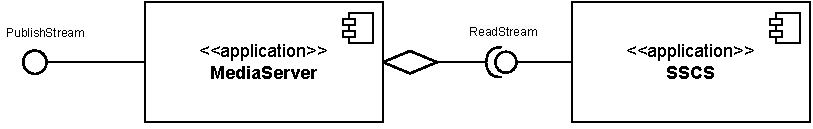
\includegraphics[width=1\linewidth]{arch1.pdf}
	\caption[Exemplo de arquitetura de transmissão]{Arquitetura de transmissão, múltiplas fontes para um servidor de mídia}
	\label{fig:graficosVariandoTamanhoRede}
\end{figure}

% \begin{figure}[!ht]
% 	\centering
% 	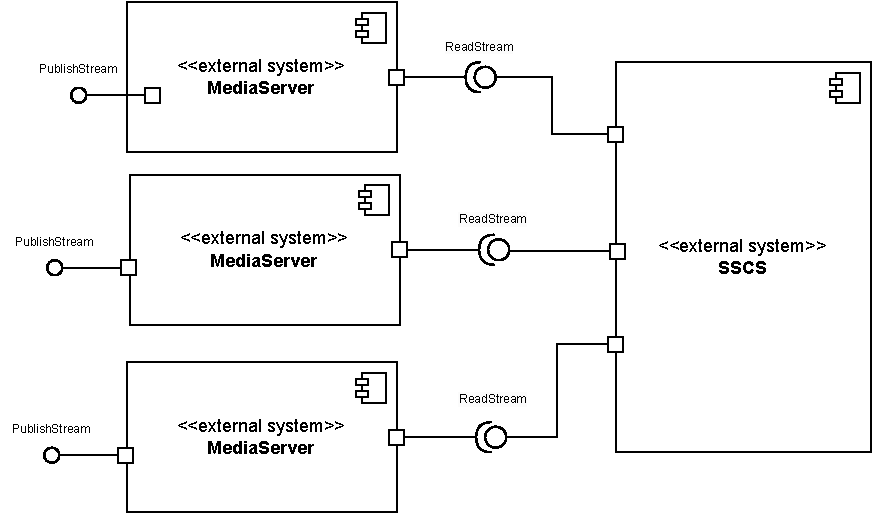
\includegraphics[width=0.8\linewidth]{arch2.pdf}
% 	\caption[Exemplo de arquiteutra de transmissão]{Arquitetura de transmissão, múltiplos servidores de mídia}
% 	\label{fig:graficosVariandoTamanhoRede}
% \end{figure}

A imagem mostra a configuração básica do SSCS, onde câmeras ou outras fontes de
transmissão de multimídia podem encaminhar fluxos para um servidor
intermediário. Esse servidor de mídia intermediário disponibiliza uma interface
chamada PublishStream, que possibilita a recepção de fluxos de multimídia de
diversas origens distintas. O símbolo em forma de losango indica que o
MediaServer age como um agregador, o que significa que ele pode interagir
simultaneamente com várias aplicações do SSCS. Contudo, é importante observar
que essa conexão é de natureza flexível: o MediaServer pode operar de forma
independente, sem depender do SSCS.

Os servidores intermediários desempenham o papel de proxies para o servidor que
opera o SSCS. A utilização de um servidor de mídia como proxy apresenta
diversas vantagens. Por exemplo, pode ser necessário converter o protocolo de
transmissão de RTSP para WebRTC ou HLS, realizar balanceamento de carga, ou até
mesmo implementar autenticação externa.

À seguir, será apresentada uma visão geral de cada componente do sistema, sua função, como ele interage
com as outras partes do sistema e detalhes de implementação. Note que cada componente é abstrato. Ou seja,
é uma base que deve ser adaptada de acordo com os protocolos, formato de imagem, banco de dados e outros detalhes
específicos de implementação. Em cada seção, há também exemplos de implementações acrescentando os detalhes.

\section{Gerenciador de Configuração}

O Gerenciador de Configuração atua na administração de variáveis de ambiente,
essenciais para distinguir entre diferentes contextos operacionais, como
desenvolvimento, teste e produção. Utilizando arquivos \texttt{.yaml} para
definir estas variáveis, o sistema ganha em flexibilidade e segurança, pois
permite a personalização do comportamento da aplicação sem alterações diretas
no código-fonte. Assim, parâmetros sensíveis podem ser injetados no ambiente de
execução, escondendo informações críticas e facilitando a adaptação do sistema
a mudanças de requisitos ou infraestrutura.

Essa função do software, embora não constitua um componente por si só, serve
como um recurso reutilizável que pode ser importado por diferentes partes do
sistema. Sua implementação é bem sucinta, como mostra o código à seguir. Nele,
o método \mintinline{go}{findConfig()} procura o arquivo \texttt{sscs.yml} em
algumas localizações comuns diferentes e devolve a primeira que encontrar.

\begin{minted}
	[%
	 breaklines,
	 mathescape,
	 linenos,
	 numbersep=5pt,
	 frame=single,
	 numbersep=5pt,
	 xleftmargin=0pt,
	 ]{go}
func ReadConf() (Config, error) {
	cfg, err := findConfig()
	return cfg, err
}
\end{minted}

\section{Gravador}

Esse é o componente principal do sistema. Sua função básica consiste em em
receber pacotes da corrente de vídeo por meio de algum protocolo de rede,
concatená-los e codificá-los em um arquivo único, com subsequente armazenamento
no disco ou nuvem em segmentos de arquivos. Estes arquivos são registrados com
uma timestamp, refletindo o instante de criação do arquivo de gravação.

Assim como a maioria dos outros componentes desse sistema, o gravador precisa
implementar todas as funções de uma interface padrão, à seguir. Os métodos
\mintinline{go}{Start()}, \mintinline{go}{Stop()} e
\mintinline{go}{setupLogger()} fazem parte de qualquer componente. Os dois
primeiros são evidentemente usados para iniciar e parar o serviço. O método
\mintinline{go}{setupLoogger()} por sua vez cria um padrão de logs customizado
para aquele componente. Isso facilita a depuração de problemas e performance.
Os últimos dois ficam á critério da implementação.

\begin{minted}
	[%
	 breaklines,
	 mathescape,
	 linenos,
	 numbersep=5pt,
	 frame=single,
	 numbersep=5pt,
	 xleftmargin=0pt,
	 ]{go}
type Recorder interface {
	Start() error 
	Stop() error 
	setupLogger()
	record() error
	sendFrame(image.Image) error
}

type EventChannels struct {
	RecordOut chan<- RecordedEvent
	FrameOut  chan<- image.Image
}	

type Config struct {
	rtspFeed string
}
\end{minted}

No contexto do desenvolvimento em Go, o método \mintinline{golang}{record}
implementado pelo componente \texttt{Recorder} é privado, o que significa que
sua acessibilidade se restringe ao pacote onde foi declarado. Esse método
realiza o consumo de uma corrente de dados exposta por um servidor de mídia. Na
prática, uma entidade do tipo \texttt{MediaServer} fornece uma interface para
que o \texttt{Recorder} desempenhe suas operações. A gravação também não é
exclusiva a um protocolo específico: qualquer sistema que tenha a capacidade de
transmitir mídia utilizando os protocolos RTSP, WebRTC ou SRT pode ser
integrado também, assumindo que o componente de gravador dê suporte.

Para comunicar aos outros componentes que um segmento foi gravado no
armazenamento, utiliza-se a interface provida \texttt{RecordedEvent}, que
encapsula informações como o tempo de início e término da gravação. Esta
estrutura compartilhada é transmitida através do canal com buffer
\texttt{RecordOut}, permitindo assim que o gravador continue seu processo sem
aguardar a finalização do indexador para cada evento de gravação. Em contraste,
se um canal sem buffer fosse utilizado, o gravador necessitaria esperar pela
conclusão da indexação de cada evento antes de iniciar a gravação subsequente,
resultando em uma sincronização mais rígida e potencialmente uma latência maior
no sistema, o que seria menos vantajoso em questões de performance. O canal
\texttt{FrameOut}, por sua vez, recebe quadros individuais. Isso é útil para os
componentes reconhecedores de imagem que podem processar esses quadros.

O método \texttt{sendFrame} é usado para alocar quadros no canal
\texttt{FrameOut}. Em relação a comunicação com outros componentes, seu
funcionamento é semelhante ao da interface anterior, utilizando também um canal
com buffer. A diferença está apenas no tamanho do buffer do canal. A
responsabilidade dessa função é pegar quadros recebidos pelo gravador e
enviá-los para a leitura por detectores de imagem.

Esse componente aceita como configuração uma URL de um servidor de mídia que
utiliza o protocolo RTSP para transmissão de dados de mídia.

\begin{figure}[!ht]
	\centering
	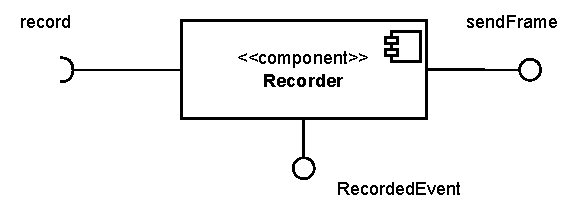
\includegraphics[width=0.7\linewidth]{gravador.pdf}
	\caption[Diagram isolado do gravador]{Diagram isolado do gravador}
	\label{fig:graficosVariandoTamanhoRede}
\end{figure}

\subsection{Implementação de gravador com RTSP e compressão H.264}

Considerando a prevalência do protocolo RTSP e do codec de compressão H.264 no
universo das câmeras IP, é fundamental que o SSCS empregue essas tecnologias em
seu gravador. Essa implementação utiliza um cliente RTSP, um multiplexador para
converter quadros H.264 em um arquivo MPEG-TS e um decodificador para extrair
quadros de vídeo.

\begin{figure}[!ht]
	\centering
	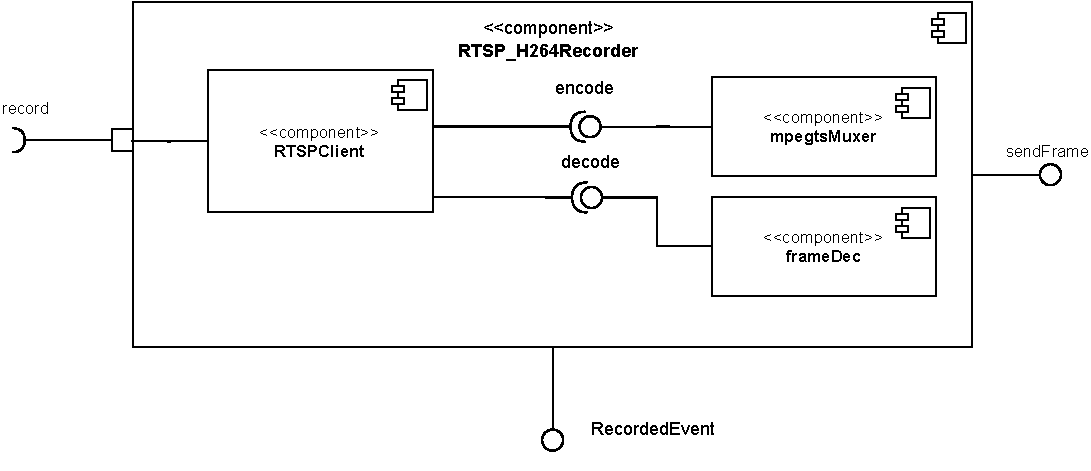
\includegraphics[width=1\linewidth]{rtsp_h264recorder.pdf}
	\caption[Diagrama isolado do gravador RTSP]{Diagrama isolado do gravador RTSP}
	\label{fig:graficosVariandoTamanhoRede}
\end{figure}

O cliente RTSP primeiro emite um requisição do tipo DESCRIBE ao servidor de
mídia, que por sua vez responde com a descrição dos dados da sessão, de acordo
com o protocolo SDP. Essa descrição contém as informações necessárias para
iniciar o streaming.

Em seguida, o cliente processa cada pacote RTP recebido e extrai as Access
Unities (AUs). Essas, são formadas por um conjunto de unidades de Network
Abstraction Layer (NAL) sempre contendo uma imagem codificada primária,
tipicamente um quadro do tipo I. Além da imagem codificada primária, uma AU
também pode conter uma ou mais imagens codificadas redundantes ou outras
unidades NAL que não contenham fatias ou partições de dados de fatias de uma
imagem codificada. A decodificação de uma AU sempre resulta em uma imagem
decodificada. Por isso, as AUs são passadas para o multiplexador que codifica
elas e organiza as unidades NAL para formar um único segmento de vídeo e
salvá-lo no disco.

O decodificador que extrai quadros de vídeo faz isso iterando as unidades NAL
até encontrar um Quadro I, que contém uma imagem completa. Quando encontrado,
ele usa o método \mintinline{go}{sendFrame()} para comunicar a imagem à um
canal com buffer. A intenção nisso é facilitar a comunicação com a parte do
software que realiza o reconhecimento de imagem em tempo real.

Por último, uma canal que recebe exclusivamente interface
\mintinline{go}{RecordedEvent} será alimentado toda vez que uma gravação for
concluída, contendo o nome do vídeo e uma timestamp do fim da gravação. Isso
pode ser usado para comunicar o registro de cada arquivo à outros componente do
sistema.

\section{Indexador}

O indexador é responsável por fazer referências aos vídeos em um banco de dados
e salvar eventos de reconhecimento de imagem. Posteriormente, exploraremos como
o indexador interage com uma API que simplifica e expande o processo de busca e
recuperação de gravações. É importante salientar também que a implementação do
indexador não se torna mandatória, a menos que corresponda a uma necessidade
específica do usuário.

A interface do indexador é bem mais simplificada. Ele requer apenas um método
privado, chamado \mintinline{go}{listen()}. A única função desse método é
esperar por eventos de indexação enviados pelos canais de outros componentes e
encaminhá-los para as funções que lidam o registro da informação no banco de
dados.

\begin{minted}
	[%
	 breaklines,
	 mathescape,
	 linenos,
	 numbersep=5pt,
	 frame=single,
	 numbersep=5pt,
	 xleftmargin=0pt,
	 ]{go}
type Indexer interface {
	Start() error
	Stop() error
	setupLogger()
	listen() error
}
\end{minted}

No diagrama à seguir, mostra-se que o indexador não provê nenhuma interface,
ele apenas requer algumas. Isso porque ele lida exclusivamente com a escrita
das informações que recebe por meio dos eventos recebidos por meio dos canais.
Um detalhe pertinente é o fato do indexador ser agnóstico quanto ao banco de
dados usado. Do ponto de vista da arquitetura, o banco de dados é uma
não-entidade. É um detalhe que não se eleva ao nível de um elemento
arquitetônico. Ele é uma utilidade que provê acesso aos dados. No mesmo ponto
de vista, essa utilidade é irrelevante pois é um detalhe de baixo nível, ou
seja, um mecanismo. \cite{martin2018clean}

\begin{figure}[!ht]
	\centering
	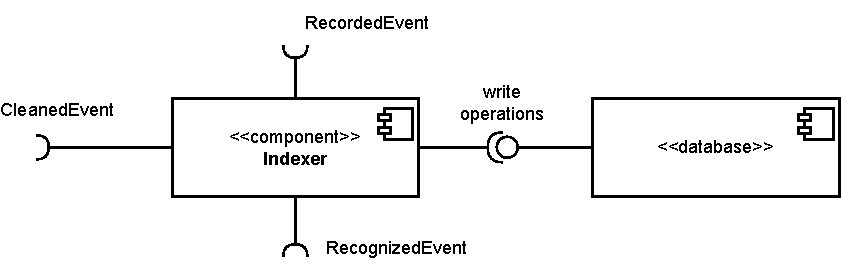
\includegraphics[width=0.8\linewidth]{indexer.pdf}
	\caption[Diagrama isolado do indexador]{Diagrama isolado do indexador}
	\label{fig:graficosVariandoTamanhoRede}
\end{figure}

\subsection{Implementação do indexador com PostgreSQL}
Bancos de dados relacionais são normalmente utilizados para indexação de dados,
e nesta implementação optou-se pelo PostgreSQL. A interação com o banco é
simplificada através do ORM GORM \cite{gorm}, que abstrai os eventos para
persistência nas tabelas e facilita migrações automáticas. Essas migrações
sincronizam a estrutura do banco com os modelos Go, agilizando o
desenvolvimento ao dispensar scripts SQL. No entanto, em ambientes de produção,
recomenda-se desativar as migrações automáticas para evitar alterações não
testadas.

\begin{figure}[!ht]
	\centering
	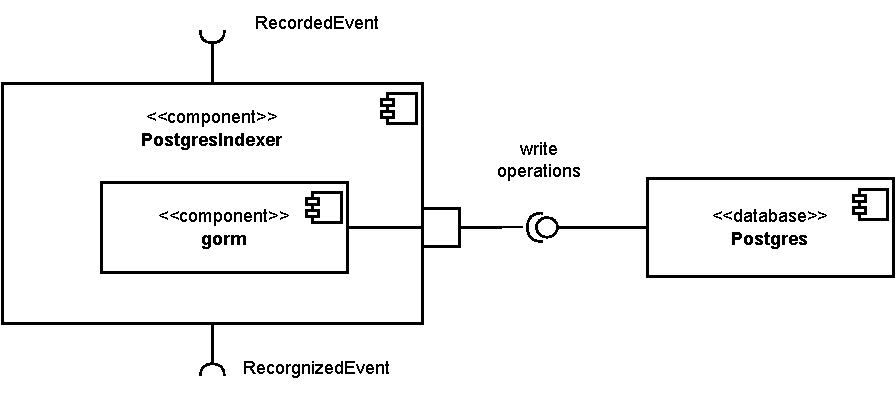
\includegraphics[width=1\linewidth]{postgres_indexer.pdf}
	\caption[Diagrama isolado da implementação do indexador com PostgreSQL]{Diagrama isolado da implementação do indexador com PostgreSQL}
	\label{fig:graficosVariandoTamanhoRede}
\end{figure}

\section{Reconhecedor}
Esse componente tem como responsabilidade analisar as correntes de vídeo
recebidas e identificar padrões ou objetos específicos. Após a captura dos
pacotes de vídeo através de um protocolo de rede, o reconhecedor processa cada
quadro individualmente, aplicando modelos de inteligência artificial ou
aprendizado de máquina.

A informação adquirida pelo reconhecedor pode ser utilizada para diversas
finalidades, como análise comportamental, detecção de intrusos, reconhecimento
facial, entre outros. A saída processada normalmente inclui metadados
associados a cada imagem reconhecida, tais como categoria do evento
reconhecido, timestamp e enquadramento da figura reconhecida.

\begin{minted}
	[%
	 breaklines,
	 mathescape,
	 linenos,
	 numbersep=5pt,
	 frame=single,
	 numbersep=5pt,
	 xleftmargin=0pt,
	 ]{go}
type Recognizer interface {
	Start() error
	Stop() error
	setupLogger()
	view() error
}
\end{minted}

Assim como o indexador, essa interface é simplificada. Há apenas um método
privado, o \texttt{view}, que lida com o processamento de cada imagem. As
imagens são consumidas em um canal que pode ser alimentado por outros
componentes como o gravador. Por alto nível, o componente reconhecedor se
assemelha com o diagrama seguinte, onde ele provê a interface que emite eventos
de reconhecimento e necessita a integração de uma interface para ler quadros.

\begin{figure}[!ht]
	\centering
	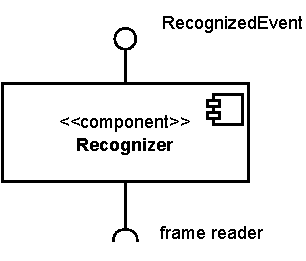
\includegraphics[width=0.4\linewidth]{recognizer.pdf}
	\caption[Diagrama isolado da implementação do reconhecedor de imagens]{Diagrama isolado da implementação do reconhecedor de imagens}
	\label{fig:graficosVariandoTamanhoRede}
\end{figure}

\subsection{Implementação de reconhecedor de movimento}
Essa implementação utiliza o algoritmo de segmentação de fundo baseado em
mistura gaussiana da biblioteca OpenCV, definido na classe
\texttt{BackgroundSubtractorMOG2}. Como o projeto está codificado na linguagem
Go, foi usado o pacote gocv, que encapsula o OpenCV para facilitar a interação
\cite{gocv_package}.

De maneira resumida, essa implementação primeiro diferencia o plano de fundo do
primeiro plano usando o algoritmo citado anteriormente. Após a separação,
ocorre uma limpeza utilizando a técnica de limiarização (thresholding) na
imagem resultante da diferenciação. O resultado disso é uma imagem binária,
onde todos os pixels acima de um valor de limiar são definidos para um valor
máximo e todos os outro para zero. Em seguida, ocorre a dilatação, que expande
as áreas brancas (também chamadas de áreas de movimento) da imagem conectando
regiões próximas e preenchendo lacunas, o que simplifica a próxima etapa, que é
inserção de contornos.

\section{Gerenciador de armazenamento}
As câmeras de segurança geralmente operam em vigilância contínua, o que
significa que elas podem produzir uma quantidade significativa de dados de
mídia. Dado que o espaço de armazenamento é um recurso custeado e limitado,
seja em dispositivos locais ou em soluções baseadas em nuvem, é crucial
implementar estratégias eficazes de gerenciamento de armazenamento.

Nesse sentido, foi criado o componente \texttt{Storer}. Sua função é justamente
monitorar o armazenamento em períodos de tempo, apagando ou movendo os arquivos
mais antigos para que um limite do armazenamento primário não seja excedido. Ao
deletar ou mover para o armazenamento secundário, ele também provê o evento
\texttt{CleanedEvent}, por meio de um canal \texttt{CleanOut}, que descreve os
arquivos e a ação para que componentes como o indexador possam deletar as
referências aos arquivos.

\begin{minted}
	[%
	 breaklines,
	 mathescape,
	 linenos,
	 numbersep=5pt,
	 frame=single,
	 numbersep=5pt,
	 xleftmargin=0pt,
	 ]{go}
type Storer interface {
	Start() error
	Stop() error
	setupLogger()
	monitor() error
	OpenFiles(filenames []string) ([]*os.File, error)
}	

type EventChannels struct {
	CleanOut chan<- CleanedEvent
}

type Config struct {
	sizeLimit   int
	checkPeriod int
	folderPath  string
	backupPath  string
}

type FileStatus int

const (
	FileUnchanged FileStatus = iota // File remains unchanged
	FileMoved                       // File was moved
	FileErased                      // File was erased
)

type CleanedEvent struct {
	filename   string
	fileSize   int
	fileStatus FileStatus
}
\end{minted}

Por meio dos método \texttt{monitor} demonstrado na interface acima, é ativada
a rotina periódica do \texttt{Storer} descrita no parágrafo anterior. Além
desse método e dos outros métodos padrões de componente, há o método
\mintinline{go}{OpenFiles} que lida com a busca e abertura dos arquivos por
meio de seus nomes. Isso é útil para outros componentes ou aplicações que
precisem filtrar arquivos de mídia específicos.

Existem quatro configurações disponíveis para o \texttt{Storer}. um inteiro que
representa o limite do tamanho do diretório em bytes, \texttt{sizeLimit}. Um
outro inteiro que representa o período de checagem do tamanho do armazenamento
em segundos, \texttt{checkPeriod}. Por último, duas strings que representam
respectivamente os diretórios de armazenamento primário e backup,
\texttt{folderPath} e \texttt{backupPath}.

\begin{figure}[!ht]
	\centering
	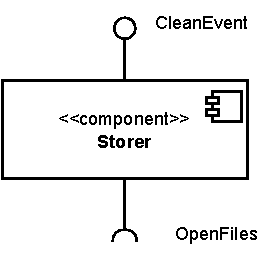
\includegraphics[width=0.3\linewidth]{storer.pdf}
	\caption[Diagrama isolado da implementação do gerenciador de armazenamento]{Diagrama isolado da implementação do gerenciador de armazenamento }
	\label{fig:graficosVariandoTamanhoRede}
\end{figure}

\subsection{Implementação de gerenciador de armazenamento sobre espaço em disco}
Nesta implementação, são usados comandos do sistema operacional para mover ou
deletar os arquivos. Checa-se primeiro o espaço acumulado de todos os arquivos
do diretório primário escolhido para armazenamento das gravações. Em seguida,
eles são ordenados por data de criação e os mais antigos podem ser movidos ou
apagados, dependendo de como o componente foi configurado.

\begin{figure}[!ht]
	\centering
	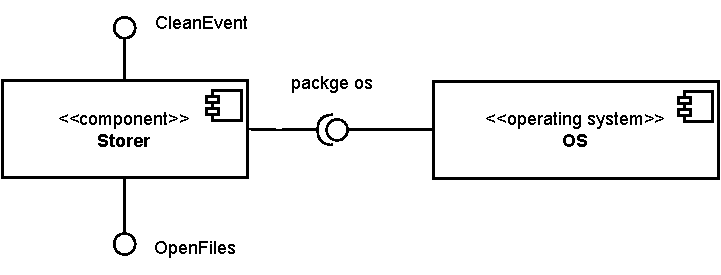
\includegraphics[width=0.8\linewidth]{storer_os.pdf}
	\caption[Diagrama da implementação do gerenciador de armazenamento usando o sistema operacional]{Diagrama da implementação do gerenciador de armazenamento usando o sistema operacional }
	\label{fig:graficosVariandoTamanhoRede}
\end{figure}

\section{API Web}

\section{Interface gráfica}

\section{Documentação}
A documentação é fundamental para tornar o software acessível e simplificar sua
manutenção. Ela deve ser clara, precisa e fácil de gerar. Idealmente, deve
estar integrada ao próprio código, para que a documentação evolua juntamente
com ele. Quanto mais fácil for para os programadores produzirem uma boa
documentação, melhor para todos.

Nesse sentido, para o código do SSCS a melhor ferramenta documentativa é a
\texttt{godoc}, que já vem integrada do toolchain do Go. A \texttt{godoc}
examina os arquivos de código Go, extrai os comentários e organiza-os em uma
documentação legível, seja como HTML ou como texto puro. Essa abordagem
assegura que a documentação esteja fortemente acoplada com o código que ela
descreve, refletindo as convenções de comentários do Go e simplificando a
navegação e compreensão do código para outros desenvolvedores.

As convenções de comentários do Go são fáceis de lembrar também. Para comentar
um tipo, variável, constante, função ou pacote, escreva o comentário
diretamente antes de sua declaração, sem linhas em branco. A \texttt{godoc}
então será capaz de apresentar o comentário junto com o item que está sendo
documentado. Veja como exemplo um comentário do pacote \texttt{recognizer} do
SSCS:

\begin{minted}
	[%
	 breaklines,
	 mathescape,
	 linenos,
	 numbersep=5pt,
	 frame=single,
	 numbersep=5pt,
	 xleftmargin=0pt,
	 ]{go}
// Package recognizer provides implementations
// for multiple image recognition algorithms.
package recognizer
\end{minted}

Note que o comentário começa com o nome do elemento que está descrevendo. É
essa convenção simples que permite gerar documentos em uma vários formatos,
como páginas web, texto plano ou páginas \texttt{man} do UNIX. Ou seja, se for
preciso visualizar a documentação de um módulo direto no terminal, uma das
maneiras é usar o comando \texttt{go doc}, da seguinte maneira:

\begin{minted}
	[%
	 breaklines,
	 mathescape,
	 linenos,
	 numbersep=5pt,
	 frame=single,
	 numbersep=5pt,
	 xleftmargin=0pt,
	 ]{bash}
$  go doc  github.com/pedrohba1/SSCS/services/recognizer  	 
package recognizer // import "github.com/pedrohba1/SSCS/services/recognizer"

Package recognizer provides implementations for multiple image recognition algorithms.


type CompositeRecognizer struct{ ... }
    func MewCompositeRecognizer(fchan chan image.Image) *CompositeRecognizer
type FaceDetector struct{ ... }
    func NewFaceDetector(fchan chan image.Image) *FaceDetector
type MotionDetector struct{ ... }
    func NewMotionDetector(fchan chan image.Image) *MotionDetector
type Recognizer interface{ ... }
\end{minted}

Analogamente, se for preferível páginas web para navegar pela documentação, uma
instância de servidor web local da \texttt{godoc} pode ser iniciada localmente
por meio da execução do comando \mintinline{bash}{ godoc -http=:6060} na raiz
do módulo. Além disso, a documentação pode ser publica online no domínio da
central de documentações do Go, \texttt{pkg.go.dev}, desde que as tags de
versão sejam usadas no repositório contendo o código. pacotes da linguagem Go.
Inclusive, o SSCS tem sua documentação toda disponível em
\url{https://pkg.go.dev/github.com/pedrohba1/SSCS/services}.

% ---
% Conclusão
% ---
\chapter[Conclusão]{Conclusão}
%TCC:
Esse trabalho detalhou o processo de desenvolvimento do SSCS, suas qualidades

% ----------------------------------------------------------
% ELEMENTOS PÓS-TEXTUAIS
% ----------------------------------------------------------
\postextual

% ----------------------------------------------------------
% Referências bibliográficas
% ----------------------------------------------------------
\bibliography{abntex2-modelo-references}

%% ----------------------------------------------------------
%% Apêndices TCC: só mantenha se for pertinente.
%% ----------------------------------------------------------

% ---
% Inicia os apêndices
% ---
% \begin{apendicesenv}

% 	% Imprime uma página indicando o início dos apêndices
% 	\partapendices

% 	% ----------------------------------------------------------
% 	\chapter{Quisque libero justo}
% 	% ----------------------------------------------------------

% 	\lipsum[50]

% 	% ----------------------------------------------------------
% 	\chapter{Coisas que fiz e que achei interessante mas não tanto para entrar no corpo do texto}
% 	% ----------------------------------------------------------
% 	\lipsum[55-57]

% \end{apendicesenv}
% ---

% ----------------------------------------------------------
% Anexos %TCC: so mantenha se pertinente.
% ----------------------------------------------------------

% ---
% Inicia os anexos
% ---
% \begin{anexosenv}

% 	% Imprime uma página indicando o início dos anexos
% 	\partanexos

% 	% ---
% 	\chapter{Eu sempre quis aprender latim}
% 	% ---
% 	\lipsum[30]

% 	% ---
% 	\chapter{Coisas que eu não fiz mas que achei interessante o suficiente para colocar aqui}
% 	% ---

% 	\lipsum[31]

% 	% ---
% 	\chapter{Fusce facilisis lacinia dui}
% 	% ---

% 	\lipsum[32]

% \end{anexosenv}

%---------------------------------------------------------------------
% INDICE REMISSIVO
%---------------------------------------------------------------------

\printindex

\end{document}